\documentclass[12pt]{article}
\usepackage[utf8]{inputenc} % allow utf-8 input
\usepackage[T1]{fontenc}    % use 8-bit T1 fonts
\usepackage{lmodern}
\usepackage{hyperref}       % hyperlinks  %[implicit=false, bookmarks=false]
\usepackage{url}            % simple URL typesetting
\usepackage{booktabs}       % professional-quality tables
\usepackage{amsfonts}       % blackboard math symbols
\usepackage{nicefrac}       % compact symbols for 1/2, etc.
\usepackage{microtype}      % microtypography
\usepackage[margin=1.0in]{geometry}

\usepackage{mathtools, amsmath, amssymb, amsthm, graphicx, verbatim}
%\usepackage[thmmarks, thref, amsthm]{ntheorem}
\usepackage{color}
\definecolor{darkblue}{rgb}{0.0,0.0,0.2}
\hypersetup{colorlinks,breaklinks,
            linkcolor=darkblue,urlcolor=darkblue,
            anchorcolor=darkblue,citecolor=darkblue}
\usepackage{wrapfig}
\usepackage{subcaption}
\usepackage[colorinlistoftodos,textsize=tiny]{todonotes} % need xargs for below
%\usepackage{accents}
\usepackage{bbm}
\usepackage{xspace}

\usetikzlibrary{calc}
\newcommand{\Comments}{1}
\newcommand{\mynote}[2]{\ifnum\Comments=1\textcolor{#1}{#2}\fi}
\newcommand{\mytodo}[2]{\ifnum\Comments=1%
  \todo[linecolor=#1!80!black,backgroundcolor=#1,bordercolor=#1!80!black]{#2}\fi}
\newcommand{\raf}[1]{\mynote{green}{[RF: #1]}}
\newcommand{\raft}[1]{\mytodo{green!20!white}{RF: #1}}
\newcommand{\jessie}[1]{\mynote{purple}{[JF: #1]}}
\newcommand{\jessiet}[1]{\mytodo{purple!20!white}{JF: #1}}
\newcommand{\bo}[1]{\mynote{blue}{[Bo: #1]}}
\newcommand{\botodo}[1]{\mytodo{blue!20!white}{[Bo: #1]}}
\ifnum\Comments=1               % fix margins for todonotes
  \setlength{\marginparwidth}{1in}
\fi


\newcommand{\reals}{\mathbb{R}}
\newcommand{\posreals}{\reals_{>0}}%{\reals_{++}}
\newcommand{\dom}{\mathrm{dom}}
\newcommand{\epi}{\text{epi}}
\newcommand{\relint}{\mathrm{relint}}
\newcommand{\prop}[1]{\Gamma[#1]}
\newcommand{\eliccts}{\mathrm{elic}_\mathrm{cts}}
\newcommand{\eliccvx}{\mathrm{elic}_\mathrm{cvx}}
\newcommand{\elicpoly}{\mathrm{elic}_\mathrm{pcvx}}
\newcommand{\elicembed}{\mathrm{elic}_\mathrm{embed}}

\newcommand{\cell}{\mathrm{cell}}

\newcommand{\abstain}[1]{\mathrm{abstain}_{#1}}
\newcommand{\mode}{\mathrm{mode}}

\newcommand{\simplex}{\Delta_\Y}

% alphabetical order, by convention
\newcommand{\C}{\mathcal{C}}
\newcommand{\D}{\mathcal{D}}
\newcommand{\E}{\mathbb{E}}
\newcommand{\F}{\mathcal{F}}
\newcommand{\I}{\mathcal{I}}
\newcommand{\R}{\mathcal{R}}
\newcommand{\U}{\mathcal{U}}
\newcommand{\X}{\mathcal{X}}
\newcommand{\Y}{\mathcal{Y}}
\renewcommand{\P}{\mathcal{P}}

\newcommand{\risk}[1]{\underline{#1}}
\newcommand{\inprod}[2]{\langle #1, #2 \rangle}%\mathrm{int}(#1)}
\newcommand{\inter}[1]{\mathrm{int}(#1)}%\mathrm{int}(#1)}
%\newcommand{\expectedv}[3]{\overline{#1}(#2,#3)}
\newcommand{\expectedv}[3]{\E_{Y\sim{#3}} {#1}(#2,Y)}
\newcommand{\toto}{\rightrightarrows}
\newcommand{\strip}{\mathrm{strip}}
\newcommand{\trim}{\mathrm{trim}}
\newcommand{\fplc}{finite-piecewise-linear and convex\xspace} %xspace for use in text
\newcommand{\conv}{\mathrm{conv}}
\newcommand{\indopp}{\bar{\mathbbm{1}}}
\newcommand{\ones}{\mathbbm{1}}
\DeclarePairedDelimiter\ceil{\lceil}{\rceil}

\newcommand{\Ind}[1]{\mathbf{1}\{#1\}}

\DeclareMathOperator*{\argmax}{arg\,max}
\DeclareMathOperator*{\argmin}{arg\,min}
\DeclareMathOperator*{\arginf}{arg\,inf}
\DeclareMathOperator*{\sgn}{sgn}

\newtheorem{theorem}{Theorem}
\newtheorem{lemma}{Lemma}
\newtheorem{proposition}{Proposition}
\newtheorem{definition}{Definition}
\newtheorem{corollary}{Corollary}
\newtheorem{conjecture}{Conjecture}
\newtheorem{claim}{Claim}


\title{Embedding characterization-- fixing a report}
\date{}

\begin{document}
\maketitle
\section{Preliminaries}
\subsection*{Notation}
Let $\gamma:\simplex \toto \R$ be a finite, nondegenerate, elicitable property, i.e. $|\R| = m < \infty$ and $\gamma(p) \neq \emptyset$ for all $p \in \simplex$.

For $p \in \simplex$, we denote polytope $T(r,p) := \sum_{y \in \Y}p_y T(r,y)$, where summation is the weighted Minkowski sum.

\subsection*{Background}
We know from Lambert 09 and 18 that the cells $\{\gamma_r\}_{r \in \R}$ form a power diagram, or equivalently, a Voronoi diagram restricted to $\simplex$.
This implies that each level set $\gamma_r$ is a convex polytope.
It has been established each polytope has both an $H$-representation (halfspace; written as matrix inequality) and a $V$-representation (vertex; written as the convex hull of a finite set of vertices).

We fix some report $r \in \R$ and focus on its level set $\gamma_r$.
Again, since $\gamma$ is a finite, elicitable property, we know that $\gamma_r$ is a convex polytope.
By existence of the $H$-representation of $\gamma_r$, we know there is a matrix $B^r \in \reals^{k \times n}$ and vector $b \in \reals^k$ so that $\gamma_r = \{p \in \simplex : B^r p \geq b\}$.
In fact, we will fix $b = \vec 0$, and we will construct $B^r$ accordingly.
The intuition for this is that infinitely many hyperplanes in $\reals^n$ will intersect the $(n-1)$-dimensional simplex.
To take a unique hyperplane, we say that we want the hyperplane that intersects the origin, which is defined by taking $b = \vec 0$.


\section{Level sets to loss functions}
While having the property we want to work with is great, our end goal is to end up constructing a [probably polyhedral] loss function that elicits such a property.
We know there are two conditions that must be true in order for any loss $L$ to embed $\gamma$: optimality and monotonicity.

These conditions are stated formally below, and justified in the following subsections.
\begin{theorem}[COLT paper Theorem approx 25]
A finite property is $d$-embeddable if and only if there exist polytopes $T(r,y)$ such that the following two conditions hold:
\begin{enumerate}
	\item (Optimality.) For all $r \in \R$ and $p \in \simplex$, we have $r \in \gamma(p) \iff \vec 0 \in T(r,p)$.
	\item (Monotonicity.) There exists an embedding $\varphi:\R \to \reals^d$ and a set of convex functions $\{L_y: \reals^d \to \reals_+\}_{y \in \Y}$ such that for all $y \in \Y$ and $r \in \R$, we have $T(r,y) = \partial_r L_y(\varphi(r))$.
\end{enumerate}
\end{theorem}


This gives us a characterization, although not a construction, of loss functions that embed the desired property.
Our dream is to use this characterization to construct a loss function $L$ indirectly eliciting $\gamma$.  (i.e. $L$ should embed $\ell$ eliciting $\gamma$.)

For each $y \in \Y$, we will want to construct polytopes $T(r,y)$ so that the polytope $T(r,p) := \sum_{y \in \Y} p_y T(r,y)$, where the sum is the Minkowski sum, satisfies our optimality condition.
Under some mild assumptions on the domain, we can show these weighted Minkowski sums are equal to the subgradient set of the expected loss $\inprod{p}{L(\varphi(r))}$.
For all $p \in \simplex$, we will want the polytope $T(r,p)$ so that $p \in \gamma_r \iff p \in \{p \in \simplex : B^r p \geq 0\} \iff \vec 0 \in T(r,p)$.
To do this, we characterize when $x \in T(r,p) := \sum_{y \in \Y} p_y T(r,y)$, later substituting $x = \vec 0$.
Again, these polytopes $T(r,y)$ become the subgradient sets $\partial_r (L(r))_y$ by our Monotonicity condition.


For each face $F$ of $T(r,p)$, there is a unique decomposition of faces $F_y$ of $T(r,y)$ for each $y \in \Y$ such that $F = \sum_y p_y F_y$.\jessie{EPFLTH Theorem 3.1.2}
Each of these faces share a normal $v$ by \jessie{EPFLTH Corollary 3.1.14}, where there is a face $F_y = \{x : vx = b_y\}$.
Then $x \in T(r,p) \implies v x \leq \sum_y p_y b_y$.
Substituting $x = \vec 0$, we then see $\vec 0 \in T(r,p) \implies 0 \leq p_y b_y$ for all $y \in \Y$.
Letting the $y^{th}$ column of $B^r$ be the vector $b_y$ to enforce optimality and taking $x = 0$, we observe the construction $\vec 0 \in T(r,p) \iff B^rp \geq \vec 0$ for all such matrices $B^r$ and $p \in \simplex$.



\subsection*{Optimality}
The forward implication of the optimality condition makes sense once we think about the loss eliciting $\gamma$.
Since, in the monotonicity condition, we set $T(r,y) := \partial L_y(\varphi(r))$, then the embedded report must minimize the loss by elicitability, and therefore $\vec 0$ must be in the subgradient set.
Similarly, for the reverse implication, if $\vec 0 \in T(r,p)$ then we can see that $\varphi(r)$ minimizes the expected loss over $p$.
We can take Minkowski sums by the subdifferential sum rule\footnote{\url{https://maunamn.wordpress.com/8-the-subdifferential-sum-rule/}}, assuming $\varphi(r) \in \relint(\dom(L_y))$ for all $y \in \Y$.


This is a (finite) higher-dimensional generalization of the fact that a report $r$ is a minimizer of a function if and only if $\vec 0$ is in its subgradient set.

\subsection*{Monotonicity}
Given a finite, elicitable property $\gamma$, we know there is \emph{some} loss that elicits it.
The monotonicity condition prods us to ask what such a convex loss can look like.
For convex $L$ and $u \in \inter{\dom(L)}$, the subgradient set $\partial_r L_y(u)$ is closed and bounded\footnote{In B/V notes}; as a corollary of this fact and our monotonicity requirement\jessie{Assuming all embeddings map to the interior of the domain}, so must $T(r,y)$ be closed and bounded for all $r \in \R$ and $y \in \Y$; hence polytopes instead of polyhedra. 

%\jessie{Not in stated condition, but we want this as well.}
%In our mode example, consider distributions where $p_1 = p_2 > p_3$ for concreteness if needed.
%In this case, whatever loss function elicits the property must be flat (and minimized, by optimality) on $\conv{\{\varphi(1), \varphi(2)\}}$, so that the origin is in the subgradient sets of both $\inprod{L(\varphi(1))}{p}$ and $\inprod{L(\varphi(2))}{p}$.
%
%Moreover, we want ``adjacent'' reports to share a face of their subgradient sets for all $y \in \Y$, so that they share a face of their subgradient sets on the expected loss for the distributions where both are optimal.



\section{Halfspace representation}
Our ultimate goal is to embed a given finite property $\gamma$.
To do this, we consider necessary conditions on the subgradient sets of the loss we aim to construct, and try to relate these for the embedded reports to the geometry of the property values.

Our embedding requirements depend on the existence of some polytopes $T(r,y)$ that simultaneously satisfy optimality and monotonicity requirements.
Moreover, our goal to construct such polytopes in the lowest dimension $d$ possible.

Since each $T(r,y)$ is a convex polytope, we know it there exists $V \in \reals^{k \times d}$ and $b \in \reals^k$ such that $T(r,y) = \{x \in \reals^d : V^rx \leq b\}$.
Recall from earlier discussion that $b$ is determined by the $y^{th}$ column of $B^r$ by design.
However, $B^r$ is not unique, so we must ask what is the ``best'' $B^r$ for a given property.

In particular, by describing $\gamma_r$, it is worth asking if the constraints imposed by $\simplex$ can be assumed by the elicitability of $\gamma$ with $\dom(\gamma) = \simplex$, or if the simplex constraints need to be built into the construction of $B^r$.
This $B^r$ then dictates the vector $b$ used to describe the halfspace representation.
%From my understanding, they can be assumed, since elicitability gives us a Voronoi diagram \emph{restricted to the simplex}: an equivalent definition to a Power Diagram.
%By restricting to the simplex, we can focus on the cells of a Voronoi diagram, which are always convex polytopes.
%\jessie{Reasoning is off; flesh this out.}



Enforcing our optimality constraints brings us back to the $B^r$ matrix discussed earlier.
We aim to construct $T$ so that $r \in \gamma(p) \iff \vec 0 \in T(r,p)$ for all reports $r \in \R$ and distributions $p \in \simplex$.
Consider that $r \in \gamma(p) \iff p \in \gamma_r$, and we chose $B^r$ so that $\gamma_r = \{p \in \simplex : B^rp \geq 0\}$.
Thus, we can re-write the condition as $p \in \{q \in \simplex : B^rq \geq 0\} \iff r \in \gamma(p) \iff \vec 0 \in T(r,p)$, stated for clarity below.
\begin{align*}
\forall p \in \simplex, \; B^r p \geq 0 &\iff \vec 0 \in T(r,p)
\end{align*}

Since we have $T(r,y) := \{x \in \reals^d : V^r x \leq b\}$ for some $V^r \in \reals^{k \times d}$ and $b \in \reals^k$, which is chosen from $B^r$, we then want to ask how we should go about constructing $V^r$.

For example, we must consider that cell boundaries are not the only constraints in constructing $T(r,y)$.
Since $T(r,y)$ becomes the subgradient of $L$ at the embedding of $r$, we also restrict that $T$ must be closed and bounded.
Thus, we ask how to properly (no pun intended) restrict the construction of $T(r,y)$ so it is a polytope. \jessie{See Question 1.}

\subsection*{Example: The mode}
Consider the mode with $n=3$, whose level sets are drawn in Figure~\ref{fig:mode-simplex}.
We will revisit this as a working example throughout in order to have something concrete to visualize.

\begin{figure}
	\centering
	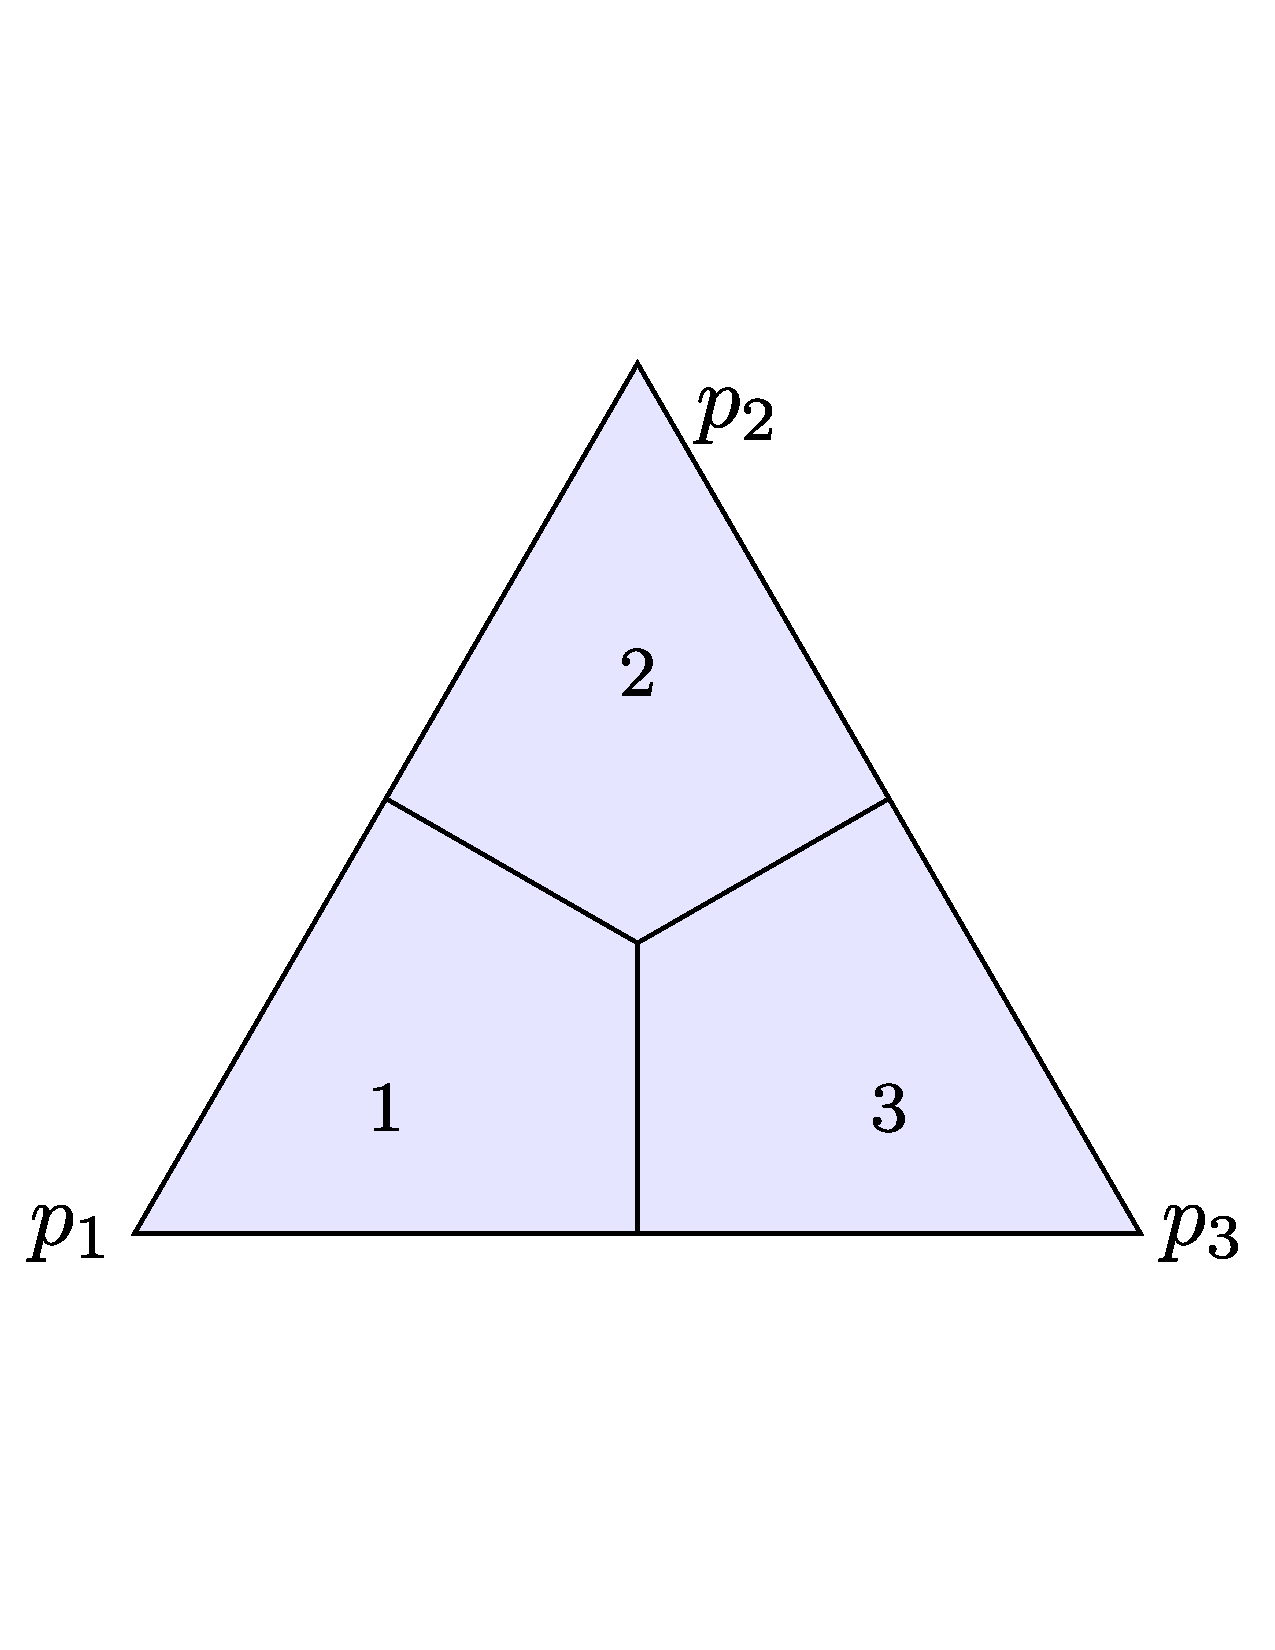
\includegraphics[width=0.5\linewidth]{figs/mode-simplex}
	\caption{Level sets of the mode $\gamma(p) = \argmax_y p_y$ with $n=3$.}
	\label{fig:mode-simplex}
\end{figure}

We can describe the cell $\gamma_1$ in one of two, nonequivalent, ways:
\[
B^1 = \{p \in \simplex: 
\begin{bmatrix}
1 & -1 & 0\\
1 & 0 & -1
\end{bmatrix} \vec p \geq \vec 0 \}
\]
or
\[
B^1 = \left\{p \in \reals^n: 
\begin{bmatrix}
1 & -1 & 0\\
1 & 0 & -1\\
0 & 1 & 0\\
0 & 0 & 1
\end{bmatrix} \vec p \geq \vec 0 \right\}
\].

These are nonequivalent since the latter doesn't include the simplex requirement that $\sum_y p_y = 1$; a constraint we cannot capture without changing the right side of the inequality to be nonzero.

\section*{``Results''}

Conditions on each $T(r,y)$ and $T(r,p)$ for all $p \in \simplex$:
\begin{enumerate}
	\item Closed and bounded (by monotonicity and subgradient characterization)
	\item Constructed with $B^r$ matrix (optimality)
	\item For all $p \in \gamma_r \cap \gamma_{r'}$, the polytopes $T(r,p)$ and $T(r',p)$ must share a face containing $\vec 0$. (monotonicity, but not as stated.)
	This suggests that the expected loss is flat on such distributions.
\end{enumerate}

One thought on restricting polytopes $T(r,y)$: for each $r \in \R$, consider the $R$ sets such that $\cap_{r' \in R} \gamma_{r'} \neq \emptyset$.
For all $p \in \cap_{r' \in R}\gamma_{r'}$, the polytopes $T(r',p)$ should share a face, possibly of a certain dimension.  (i.e. dim(level set) + dim(face) = n?) 

\section*{Questions}
\begin{enumerate}
	\item How to make the polyhedra $T(r,y)$ satisfying minimal optimality requirements be bounded? Do we do this by intersecting minimal $H$-rep with some polar, possibly $V^\circ$? 
	\item Can \emph{any} bounded polytopes $T(r,y)$ satisfying optimality and monotonicity constraints be $\partial L(r)_y$.  In other words, could the valid $T$ constructions characterize the polyhedral losses that embed $\gamma$?
	\item \jessie{Ask Nathan?} How to find $V^r$, given $B^r$ for each $r \in \R$?  Poly-time?
	\item Is there a framework where we construct $T(r,y)$ by going from H-reps to V-reps, to H-reps?  (It's computationally hard to calculate closed form of H-rep Minkowski sum, but we can just go back and forth for closed polytopes in poly time.)
	\item How does duality play into all of this?  
\end{enumerate}

\bigskip \hrule \bigskip

\section{Monotonicity and vertex representations}
Consider $\R$ to be a finite set of reports, and define $\ell:\R \times \Y \to \reals_+$.
In general, we consider $R \in 2^\R$ to be a set of elements of $\R$.

Suppose $\gamma: \simplex \toto \R$ is the finite property elicited by the discrete loss $\ell$ we wish to embed.
Take $\gamma_r = \{p \in \simplex : r \in \Gamma(p) \}$ for a single report, and $\gamma_R := \cap_{r \in R} \gamma_r$ for a set of reports $R$.

\bigskip
We want to ask: \emph{what is the relationship between $\gamma_R$, $|R|$, and $d$ for any or all $R \in 2^\R$?}
\bigskip

We assume $\gamma$ to be finite, nondegenerate, and elicitable, which informs us that $\gamma_R$ is a convex polytope for all $R$.
Therefore, for each $R \in 2^\R$, there is a unique minimal, finite set of distributions $q^R = \{q^R_1, \ldots, q^R_{k_R}\}$ so that $\gamma_R = \conv(q^R)$.
For any $p \in \gamma_R$, $p$ can be written as a convex combination of distributions in $q^R$; that is, we can write $p$ as $\sum_{i=1}^{k_R}\lambda_i q^R_i$ for $\lambda_i \in [0,1]$ and $\sum_i \lambda_i = 1$.

For convex polytope $P$, let $F(P)$ be the face lattice of $P$.
%We write $\oplus_{i=1}^{k_R}T(r, q_i^{k_R}) := T(r, \gamma_R)$, abusing notation slightly, to indicate a polytope on the relative interior (if $|q^R| >1$, and equal to $q^R$ otherwise) of the level set $\gamma_R$, up to a reweighting to which our results are agnostic.


\jessie{Future: Seems like a lot of axiom of choice... can we get rid of it?}

\begin{claim}\label{claim:face-lattice-multivalued-sets}
	$\vec 0$ is in some face of $T(r,p)$ of degree $\leq d-1$ for any $p \in \gamma_R$ such that $|R| > 1$ for all $r \in R$.
\end{claim}
\begin{proof}
	\jessie{$N(\gamma_R)$ is a positively oriented normal to the level set $\gamma_R$.}
	Consider $q := \frac{1}{1 +\epsilon_1}(p + \epsilon_1 N(\gamma_{R}))$ so that $q \in B(p, \epsilon_p)$, or the open $\epsilon_p$-ball around the distribution $p$, where we take $\epsilon_1 < \epsilon_p$.
	In particular, observe $q \not \in \gamma_r$ for some $r \in R$ since $|R|>1$ implies $\gamma_R$ is not full-dimensional in the simplex.
	
	We aim to show that $\vec 0 \not\in T(r, q)$ (from our optimality condition) implies $\vec 0$ is in a face of $T(r,p)$, and do so by proving the contrapositive.
	
	Suppose $\vec 0$ is not in a face of $T(r,p)$.
	By optimality, we must then have $\vec 0$ in the interior of $T(r,p)$.
	There is then some $\epsilon >0$ so that for all $x \in B(\vec 0, \epsilon)$, we have $x \in T(r,p)$.
	
	Since we set $q := \frac{1}{1 +\epsilon_1}(p + \epsilon_1 N(\gamma_{R}))$, we can write $T(r,q) := \frac{1}{1+\epsilon_1}T(r,p) \oplus \frac {\epsilon_1}{1 + \epsilon_1} T(r, N(\gamma_{R}))$.
	
	This second term is sufficiently close to $0$ (i.e. there is a point in the polytope also in the $\epsilon$-ball of $0$) by its weighting.  In fact, there is a point $\vec y \in \frac {\epsilon_1}{1 + \epsilon_1} T(r, N(\gamma_{R}))$ such that $\vec y \in B(\vec 0, \epsilon)$.
	We then take $\vec x := -\vec y \in \frac{1}{1 + \epsilon_1}T(r,p)$, which is also in the $\epsilon$-ball centered at $\vec 0$, so we then have $\vec 0$ in the Minkowski sum that is $T(r,q)$, thus proving our claim.
	
	\jessie{Go through and be careful about which epsilon and maintaining order of inequality}
%	For all $r \in R$, there is some $\epsilon > 0$ sufficiently small and $q \in \simplex$ such that $q \in B(p, \epsilon)$ for some $p \in \gamma_R$, but $q \in \inter{\gamma_{r}}$ for some unique $r \in R$.
%	
%	
%	We know that If $\vec 0 \in T(r',p)$ for $r' \in R$.
%	However, if $\vec 0 \in \inter{T(r',p)}$ for $r \neq r' \in R$, then we can show $\vec 0 \in T(r',q)$, contradicting our optimality condition.
%	
%	To see this, consider that \jessie{TODO...}
%	
%	Therefore, $\vec 0$ must be in a face of $T(r,p)$.
\end{proof}


Since $T(r,p)$ is a Minkowski sum of polytopes $T(r,q^R_i)$, then by \jessie{EPFLTH 3.1.4?}, there is a unique decomposition of faces of each of these polytopes so that $\vec 0$ is in each of these faces.
It is then worth making a special note that Claim~\ref{claim:face-lattice-multivalued-sets} holds for the vertices of the level set.

\bigskip
\hrule
\bigskip

The following claim assumes $|\R| > 1$ and for all $r \in \R, \gamma_r$ is full-dimensional in the relative interior of the simplex.
%\begin{claim}
%	For any $R \in 2^\R$, we have $\vec 0 \in F(T(r, \gamma_R))$ for all $r \in R$.
%\end{claim}
%\begin{proof}
%First, if $|R| > 1$, the result follows from Claim~\ref{claim:face-lattice-multivalued-sets}.
%
%If $|R| = 1$, then the same argument can be made for some of the polytopes on distributions that intersect the level sets for other reports.
%There is at most one distribution $q^R_1$ where $q^R_1 \in \gamma_r$, but $q^R_1 \not\in \gamma_{r'}$ for any $r \neq r' \in \R$.
%\jessie{Check claim?}
%In fact, this distribution, if it is in $q^R$, must be $\delta_y$ for some $y \in \Y$.
%
%In this case, we see that $\vec 0$ must be in the face of the polytope.
%Consider a distribution on the intersection of multiple level sets...?
%\jessie{Is this true?}
%
%\end{proof}

%\begin{claim}
%	For all $y \in \Y$, $\vec 0 \not \in \inter{T(r,y)}$. \jessie{Not true... take median over $\Y = \{1,2,3\}$.}
%\end{claim}
%Observe this means if $r \in \gamma(\delta_y)$, then $\vec 0$ is in a face of $T(r,y)$.
%Otherwise, $\vec 0 \not \in T(r,y)$.
%\begin{proof}
%	For $r \not \in \gamma(\delta_y)$, this follows from our optimality condition.
%	For $r \in \gamma(\delta_y)$, assuming $\gamma_r \neq \simplex$, there is a level set $\gamma_R$ with $|R| > 1$ that is nonempty.
%	Take $p \in \gamma_R$ and for a sufficiently small $\epsilon > 0$, take $q := \frac 1 {1-\epsilon} (p - \epsilon \delta_y)$. \jessie{What about $q := \frac 1 {1+\epsilon} (p + \epsilon N(\gamma_R))$?  I think original doesn't work if level set not on interior of simplex.}
%	By elicitability, we know that $r \not \in \gamma(q)$, since otherwise we would contradict convexity of level sets, so showing $\vec 0 \in T(r,q)$ contradicts optimality.
%	
%	For such a contradiction, assume $\vec 0 \in \inter{T(r,\delta_y)}$.
%	We will write $T(r,q) = \oplus_y q_y T(r,y) = \oplus_{y'} \frac 1 {1-\epsilon} p_{y'} T(r,y') + \frac{\epsilon}{1-\epsilon} T(r,y) =  \frac 1 {1-\epsilon} T(r,p) + \frac{\epsilon}{1-\epsilon} T(r,y)$.
%	
%	Since $\vec 0$ is in $T(r,p)$, it is also in the first term of this sum.
%	Since we assume $\vec 0 \in \inter{T(r,y)}$, it is also in the weighted polytope.
%	Thus, $\vec 0$ is in the sum, $T(r,q)$, yielding our contradiction.
%	
%	Therefore, we cannot have $\vec 0 \in \inter{T(r,y)}$ for all $r \in \R$ and $y \in \Y$.
%\end{proof}

\begin{definition}
	The \emph{feasible subspace dimension} $\mu_\C(p)$ of a convex polytope $\C$ at a point $p$ is the dimension of the feasible cone intersected with its negation.
\end{definition}
In essence, this is the dimension of the smallest face of $\C$ containing $p$.

\begin{conjecture}
	The dimension of the smallest face of $\sum_{i=1}^{k_R}T(r, q_i^{k_R})$ containing $\vec 0$ must be a function of $|R|$.
	Specifically, $\sum_{r \in R}\mu_{T(r,\gamma_R)}(\vec 0) \leq d$.
	Equivalently, $\sum_{r \in R} \sum_{i=1}^{k_R} \mu_{T(r,q_i)}(\vec 0) \leq d$.
\end{conjecture}
\begin{proof}
	\jessie{TODO}
\end{proof}


\section{Proper-trees}
There is a heirarchy among the report sets; if reports $r_1$ and $r_2$ are optimal, then $\Gamma_{\{r_1, r_2\}}$ must be the intersection of $\Gamma_{r_1} \cap \Gamma_{r_2}$.
So while the set-valued report set might be exponential, we can represent the level sets of a property with a tree as follows:
\begin{enumerate}
	\item At the base level, create a node for each $r \in \R$.
	\item At the next level, create up to $\binom{m}{2}$ nodes for $R \subseteq \R$ with $|R| = 2$, adding an edge from each $r \in R$ to $R$ if $\Gamma_R$ is not empty. Delete nodes that have in-degree $0$.
	\item Repeat, adding edges from the previous level to the current level, until there are no more level sets of size $h$. 
\end{enumerate}

\begin{theorem}
	Each node in the tree associated with the orderable property $\Gamma$ has in-degree at most 2.
\end{theorem}
\begin{proof}
	Orderability of the property $\Gamma$ implies the level sets are separated by hyperplanes, which can connect at most two full-dimensional levels on $\inter{\simplex}$.
	If there is $R \subseteq \R$ where $|R| > 2$ and $\Gamma_R \neq \emptyset$, then it should be able to be written as $\Gamma_{R'} \cap \Gamma_{R''}$, where $|R' \cap R''| = |R| - 1$. \jessie{Check this}
\end{proof}

\newpage

\section{Post meeting: redo}

  For any set of vectors $v_1, \ldots, v_k$ in $\reals^d$ we can organize them into the matrix $V \in \reals^{k \times d}$.  
  For any such $V$, and any polytope $T$, let $c = H_T(V) \in \reals^k$ be given by the support function for $T$ applied to each vector, i.e., $c_i = \max_{x \in T} \inprod {v_i}{x}$.  
  \begin{definition}
  	We say $V$ is \emph{complete} for $T$ if $\{x \in \reals^d : Vx \leq c\} = T$, meaning these constraints actually define $T$.   
  \end{definition}
  (It's easy to see that you always get a superset of $T$, by definition of $c$.) 
  When $T$ is full-dimensional, there is a unique set $S$ of unit normals to the facets of $T$, and $V$ is complete for $T$ if and only if $S$ is a subset of $\{v_1/\|v_1\|,...,v_k/\|v_k\| \}$.  
  When $T$ is lower-dimensional, there are even more ways to be complete.

  Now, fix a set of polytopes $T_1, \ldots, T_n$ (one for each outcome), and let us say that $V$ is complete for all of them if $V$ is complete for each $T_y$.  
  Fix such a $V$.  
  Then for all $p \in \simplex$, the $p$-weighted Minkowski sum of $T_1, \ldots, T_n$ contains $\vec 0$ if and only if $E p \geq 0$, where $E$ is the $k \times n$ matrix defined by $E_{yi} = H_{T_y}(V)_i$.

  \begin{conjecture}
	Let $T_1, \ldots, T_n$ be given such that $T := \oplus_y T_y$ is full-dimensional.
	Then $V$ is complete with respect to $T$ if and only if $V$ is complete with respect to $T_y$ for all $y$.
  \end{conjecture}

  I think the last two paragraphs are the first half of what we want to show.  
  The tricky part, which we've already figured out but still need to write carefully, is the "if and only if" bit -- this is what came from that thesis I found on Minkowski sums of polytopes.  
  For the second half, we want to relate this $E$ matrix to the $B$ we get from the cell itself.  
  Here's how Raf was picturing that.


  Let $A$ be the affine span of the simplex, i.e. $A = \{p \in \reals^d : \sum p_y = 1\}$.  
  Given a cell $C$ in the simplex, WLOG full-dimensional (otherwise the report for the discrete loss is going to be redundant), we can derive a matrix $B$ such that $\{p \in A : B p \geq 0\} = C$.  
  In fact, we can take $B$ to be unique up to permutations of the rows by insisting we derive it from unit normals to the facets of $C$, just like the comment above on full-dimensional $T$.  
  Note that if $C$ is not ``interior'' then $B$ will contain constraints for the simplex itself by the equality requirement.

  Now, we want to characterize when $E$ and $B$ represent the same cell, meaning when is it the case that $\{p \in A : B p \geq 0\} = \{p \in \simplex : E p \geq 0\} = \{p \in A : [E; I_n] \geq 0\}$.
  (Let $D := \{p \in \simplex : Ep \geq \vec 0\}$ be the cell described by $E$.)  
  Note the $A$ in the first set and simplex in the second, since we naturally think of simplex constraints being in $B$ already, but not necessarily in $E$; this is where some of the earlier confusion arose.
  
  First, observe the following: given a cell $C \subseteq \simplex$, we say that $B$ is the matrix describing it by $\{p \in A : Bp \geq \vec 0\}$.  
  We can further break that down by observing that $B$ is composed of ``interior'' constraints and simplex constraints.
  Call this matrix of interior constraints $B'$.
  We then have $\{p \in A: Bp \geq \vec 0\} = \{p \in A : [B' ; I_n] p \geq \vec 0\}$, as adding $I_n$ covers the simplex constraints not described by $B'$, while only adding redundant constraints beyond that for the other simplex constraints.
  
  Now, we can start to think about when these two cells described by $B$ and $E$ are equal.
  
  \begin{proposition}
  	Suppose we are given polytopes $T_1, \ldots, T_n$, and construct $E$ as above, and call $D = \{p \in \simplex : Ep \geq \vec 0\}$.
  	Similarly, suppose we are given a cell $C \subseteq \simplex$ and construct $B$ as above.
  	Then we have $C=D$ if and only if any row of $B'$ that is not also a row (up to invariance of scaling) of $E$ is a redundant constraint in $\{p \in \simplex: B'p \geq \vec 0\}$, and any row of $E$ that is not a (rescaled) row of $B'$ is a redundant constraint in describing $\{p \in \simplex: Ep \geq \vec 0\}$.
  \end{proposition}
  
  When $C$ is ``interior,'' meaning $\{p \in \simplex : Bp \geq 0\} = \{p \in A : Bp \geq 0\}$, or equivalently, $\{p \in A : B'p \geq \vec 0\} = \{p \in A : B p \geq \vec 0\}$, we know the rows of $B$ (possibly scaled) need to show up in $E$, but we still need to characterize in some nice way the potential other rows of $E$.  
  (That is, if I pointed out the rows that need to be there, could you easily test whether the other rows are all redundant constraints? \jessie{Redundant in what sense?  Seems like there are rows of $E$ that might be necessary for the polytopes, but are redundant in describing the cell $D$.})

  When $C$ is not interior, we have at least one simplex constraint in $B$ that does not need to show up in $E$.  
  Here we can say that some rows of $B$ (forming $B'$) must show up in $E$ (the non-simplex constraints), and for the other rows, the must be redundant when we add them to $B$ (or equivalently, when we add the simplex constraints to $E$).  
  What's not clear though is whether we can say more about what $D' = \{p \in A : E p \geq 0\}$ must look like.  
  (Note: by the above, $D' \cap \simplex = D$ \jessie{was =$C$?}, so $D'$ is the set $E$ ``really'' defines before we restrict to the simplex.)  
  In particular, is $D'$ always a polytope?  
  Statements like this one about $D'$ would really help our necessary conditions.


\end{document}
%%% Local Variables:
%%% mode: latex
%%% TeX-master: t
%%% End:
